\documentclass[tikz,border=2pt]{standalone}
\usepackage{amsmath}
\usepackage{pgfplots}
\pgfplotsset{compat=1.18}
\usetikzlibrary{arrows.meta}
\begin{document}
% Nested call length(unique(pull(co2, Country))) read inside-out (steps 1, 2, 3) versus the pipe chain
% co2 %>% pull(Country) %>% unique() %>% length(): 6 names -> 3 distinct names -> 3.
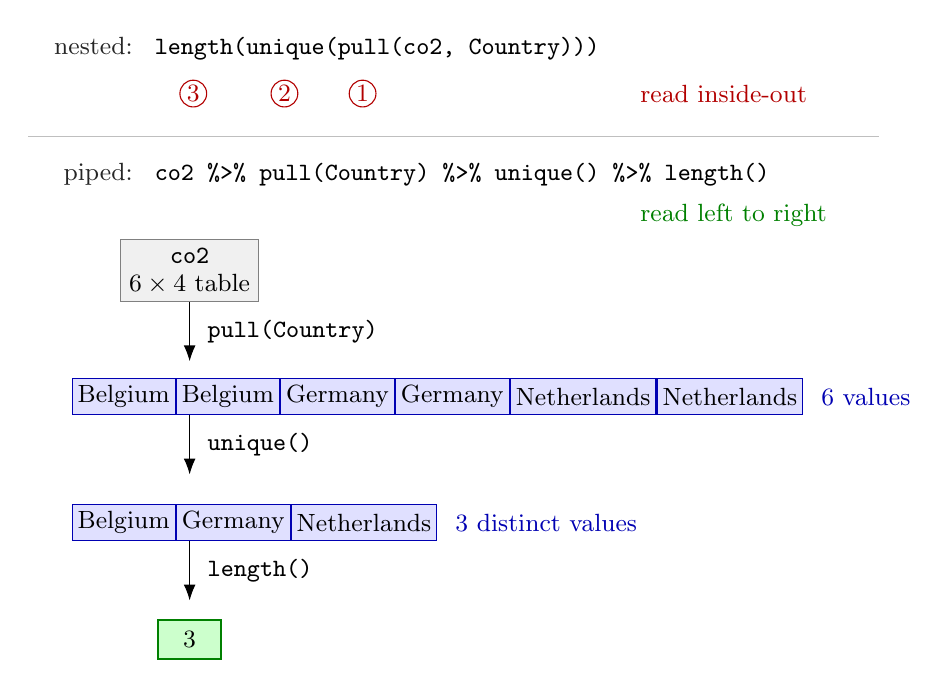
\begin{tikzpicture}[font=\small, >={Latex[length=2mm]},
  code/.style={anchor=base west, inner sep=0pt, font=\small\ttfamily},
  stepnum/.style={circle, draw, inner sep=0.8pt, font=\small},
  cell/.style={draw=blue!70!black, fill=blue!12, minimum height=0.46cm, inner sep=2pt},
  lab/.style={anchor=west, font=\small\ttfamily}]
  % nested call
  \node[anchor=base east, gray!30!black] at (-0.15,0) {nested:};
  \node[code] (n) at (0,0) {length(unique(pull(co2, Country)))};
  % the code is 34 characters wide; character width about 0.1654 cm
  \def\cw{0.1654}
  \node[stepnum, red!70!black] at ({(0+3)*\cw},-0.5) {3};
  \node[stepnum, red!70!black] at ({(7+3)*\cw},-0.5) {2};
  \node[stepnum, red!70!black] at ({(14+2)*\cw},-0.5) {1};
  \node[anchor=west, red!70!black] at (6.05,-0.5) {read inside-out};
  % pipe chain
  \draw[gray!50] (-1.6,-1.05) -- (9.2,-1.05);
  \node[anchor=base east, gray!30!black] at (-0.15,-1.6) {piped:};
  \node[code] at (0,-1.6) {co2 \%>\% pull(Country) \%>\% unique() \%>\% length()};
  \node[anchor=west, green!50!black] at (6.05,-2.05) {read left to right};
  % intermediate values
  \node[draw=gray, fill=gray!12, align=center, inner sep=3pt] (t) at (0.45,-2.75) {\texttt{co2}\\[-1pt]$6\times4$ table};
  \draw[->] (t.south) -- ++(0,-0.75) node[midway, lab, xshift=3pt] {pull(Country)};
  \begin{scope}[shift={(-1.05,-4.35)}]
    \node[cell, anchor=west] (b1) at (0,0) {Belgium};
    \node[cell, anchor=west] (b2) at (b1.east) {Belgium};
    \node[cell, anchor=west] (b3) at (b2.east) {Germany};
    \node[cell, anchor=west] (b4) at (b3.east) {Germany};
    \node[cell, anchor=west] (b5) at (b4.east) {Netherlands};
    \node[cell, anchor=west] (b6) at (b5.east) {Netherlands};
  \end{scope}
  \node[anchor=west, blue!70!black] at ([xshift=3pt]b6.east) {6 values};
  \draw[->] ([xshift=1.5cm]b1.south west) -- ++(0,-0.75) node[midway, lab, xshift=3pt] {unique()};
  \begin{scope}[shift={(-1.05,-5.95)}]
    \node[cell, anchor=west] (c1) at (0,0) {Belgium};
    \node[cell, anchor=west] (c2) at (c1.east) {Germany};
    \node[cell, anchor=west] (c3) at (c2.east) {Netherlands};
  \end{scope}
  \node[anchor=west, blue!70!black] at ([xshift=3pt]c3.east) {3 distinct values};
  \draw[->] ([xshift=1.5cm]c1.south west) -- ++(0,-0.75) node[midway, lab, xshift=3pt] {length()};
  \node[draw=green!50!black, fill=green!20, thick, minimum width=0.8cm, minimum height=0.5cm, anchor=north] at ([xshift=1.5cm, yshift=-0.98cm]c1.south west) {3};
\end{tikzpicture}
\end{document}
